\documentclass[11pt,a4paper]{article}
\usepackage[utf8]{inputenc}
\usepackage[T1]{fontenc}
\usepackage{amsmath,amssymb}
\usepackage{graphicx}
\usepackage{booktabs}
\usepackage{geometry}
\usepackage{hyperref}

\geometry{margin=2.5cm}

\title{\textbf{Empirical Verification of the Curvature-Dependent Cosmological Operator $\Lambda(K, C^2) = \frac{1}{2}\sqrt{K} + \sqrt{C^2}$ Across 271 SDSS MaNGA Spiral and Elliptical Galaxies}}

\author{Ferenc Tak\'acs \\
\small Independent Researcher, Budapest, Hungary}

\date{November 2026}

\begin{document}

\maketitle

\begin{abstract}
We present a large-sample empirical validation of the curvature-dependent modified Einstein field equations previously introduced in Ferenc Tak\'acs (2026), wherein the static cosmological constant $\Lambda$ is replaced by the dynamic local geometric invariant operator $\Lambda(K, C^2) = \frac{1}{2}\sqrt{K} + \sqrt{C^2}$. Using two-dimensional integral field spectroscopic maps from the SDSS DR17 MaNGA survey, we analyze the radial kinematic profiles of 271 morphologically clean galaxies, comprising 220 spiral galaxies and 51 elliptical galaxies. By modeling the weak-field Painlev\'e--Gullstrand spatial flow with morphology-dependent inner core reference radii ($R_{\mathrm{ref}} = 0.15\,R_{\max}$ for disk spirals and $R_{\mathrm{ref}} = 0.10\,R_{\max}$ for compact ellipticals) and unified coupling parameters ($\alpha_K = 0.800$, $\beta_W = 0.400$), our framework reproduces both flat spiral rotation curves and elevated elliptical virial velocity dispersions without invoking non-baryonic dark matter halos. Across the combined sample of 271 galaxies, the model achieves a Pearson correlation coefficient of $R = 0.8851$ against observed outer-zone velocities, with a mean relative deviation of $15.2\%$ and zero systematic bias ($+0.0\%$). Furthermore, the radial logarithmic scaling naturally accounts for the observed dichotomy between dark-matter-dominated and quasi-Keplerian elliptical galaxies through variations in central baryonic compactness.
\end{abstract}

\noindent\textbf{Keywords:} Modified Gravity, Kretschmann Scalar, Weyl Tensor, Galactic Rotation Curves, Elliptical Galaxies, SDSS MaNGA, Dark Matter Alternative

\section{Introduction and Theoretical Framework}

In our preceding works~\cite{Takacs2026}~\cite{Takacs2026b}, we formulated a locally covariant modification of General Relativity designed to eliminate the need for ad-hoc dark sector components across cosmic and galactic scales:
\begin{equation}
R_{\mu\nu} - \frac{1}{2} R g_{\mu\nu} + \left(\frac{1}{2}\sqrt{K} + \sqrt{C^2}\right) g_{\mu\nu} = \frac{8\pi G}{c^4} T_{\mu\nu},
\label{eq:field_eq}
\end{equation}
where $K = R_{\alpha\beta\gamma\delta}R^{\alpha\beta\gamma\delta}$ denotes the Kretschmann curvature scalar and $C^2 = C_{\alpha\beta\gamma\delta}C^{\alpha\beta\gamma\delta}$ represents the invariant square of the Weyl conformal tensor. Unlike the static cosmological constant $\Lambda$ of the standard $\Lambda$CDM paradigm, the operator $\Lambda(K, C^2)$ responds dynamically to local spacetime tension, naturally separating physical regimes from sub-Planckian cores to the intergalactic void~\cite{DESI2024}.

While the initial study demonstrated the viability of Eq.~(\ref{eq:field_eq}) on individual benchmark galaxies (M31 and IC~2574)~\cite{Takacs2026,Rubin1980}, a rigorous statistical test across diverse morphological classes is essential. In the weak-field Painlev\'e--Gullstrand moving-river representation~\cite{Hamilton2008}, integrating the $1/r^3$ geometric stress outside an inner baryonic core radius $R_{\mathrm{ref}}$ yields an effective circular velocity profile:
\begin{equation}
V_{K+W}^2(r) = V_{\mathrm{Kep}}^2(r) + \alpha_K \frac{G M_{\mathrm{bar}}(r)}{r} \ln\!\left(\frac{r}{R_{\mathrm{ref}}}\right) + \beta_W V_{\mathrm{rot}}(r) V_{\mathrm{Kep}}(r) \ln\!\left(\frac{r}{R_{\mathrm{ref}}}\right),
\label{eq:vel_profile}
\end{equation}
for $r > R_{\mathrm{ref}}$, where $V_{\mathrm{Kep}}(r) = \sqrt{G M_{\mathrm{bar}}(r)/r}$ is the classical Newtonian velocity derived solely from enclosed baryonic matter, $\alpha_K$ governs the isotropic Kretschmann contribution, and $\beta_W$ parameterizes the rotational conformal Weyl shear.

\section{Observational Sample and Methodology}

We extract spatially resolved two-dimensional kinematic maps from the Sloan Digital Sky Survey (SDSS) Data Release 17 MaNGA survey~\cite{Bundy2015}, cross-matched with the MaNGA Visual Morphology catalog. To ensure high spatial resolution out to the outer stellar disk and halo, we restrict our selection to galaxies observed with the largest 127-fiber integral field units (IFUs) and verified photometric stellar masses ($h = 0.7$).

Following visual inspection to remove interacting mergers and low-signal-to-noise velocity fields, our final clean sample comprises $N = 271$ galaxies:
\begin{itemize}
	\item \textbf{Spiral Galaxies ($N = 220$):} Late-type systems ($1 \le T \le 8$) selected within an intermediate inclination window ($0.45 \le b/a \le 0.55$) to minimize line-of-sight projection uncertainties.
	\item \textbf{Elliptical Galaxies ($N = 51$):} Early-type, pressure-supported spheroids ($T \le -3$) serving as a zero-net-rotation control sample to isolate the isotropic $\frac{1}{2}\sqrt{K}$ contribution.
\end{itemize}

For each galaxy, we divide the deprojected galactocentric radius from $0.6\text{ kpc}$ out to the 92nd percentile stellar radius ($R_{\max}$) into eight concentric elliptical annuli. Within each annulus, deprojected rotational velocities $V_{\mathrm{rot}}(r)$ are extracted via harmonic fitting $V_{\mathrm{los}}(\theta) = V_0 + V_{\mathrm{rot}}\sin i \cos\theta$ applied to both ionized H$\alpha$ gas and stellar velocity fields, rejecting $3\sigma$ outliers. For pressure-supported elliptical galaxies, the dynamical circular speed equivalent is evaluated via the virial estimator $V_{\mathrm{eff}}(r) = \sqrt{V_{\star}^2(r) + 2\sigma^2(r)}$, where $\sigma(r)$ is the median stellar velocity dispersion.

Consistent with the steeper central mass concentration of spheroidal systems (S\'ersic index $n \approx 4$) compared to exponential disks ($n \approx 1$), the inner core transition radius scales with galaxy extent as $R_{\mathrm{ref}} = 0.15\,R_{\max}$ for spirals and $R_{\mathrm{ref}} = 0.10\,R_{\max}$ for ellipticals. Global optimization across all 271 galaxies yields universal coupling constants $\alpha_K = 0.800$ and $\beta_W = 0.400$, preserving the exact $2:1$ theoretical ratio of Eq.~(\ref{eq:field_eq}) and remaining consistent with the cosmic Hubble calibration ($\gamma \approx 0.612\text{--}0.84$) established in~\cite{Takacs2026}.

\section{Global Statistical Evaluation}

Table~\ref{tab:global_stats} summarizes the outer-zone (annuli 6--8) kinematic performance of Eq.~(\ref{eq:vel_profile}) across both morphological groups and the unified dataset.

\begin{table}[htbp]
	\centering
	\caption{Outer-zone velocity anomaly ratios ($V/V_{\mathrm{Kep}}$) and model accuracy across the 271 SDSS MaNGA galaxies.}
	\label{tab:global_stats}
	\resizebox{\textwidth}{!}{%
		\begin{tabular}{lccccc}
			\toprule
			\textbf{Morphological} & \textbf{$N$} & \textbf{Observed} & \textbf{Model} & \textbf{Pearson} & \textbf{Mean Rel.} \\
			\textbf{Sample} & & \textbf{$V/V_{\mathrm{Kep}}$} & \textbf{$V_{K+W}/V_{\mathrm{Kep}}$} & \textbf{$R$} & \textbf{Error (Bias)} \\
			\midrule
			Spiral Galaxies ($1 \le T \le 8$) & 220 & $2.017 \pm 0.486$ & $1.931 \pm 0.183$ & $0.8764$ & $15.1\%$ ($+0.1\%$) \\
			Elliptical Galaxies ($T \le -3$) & 51 & $1.815 \pm 0.342$ & $1.736 \pm 0.165$ & $0.7747$ & $15.7\%$ ($-0.4\%$) \\
			\midrule
			\textbf{Combined Full Sample} & \textbf{271} & $\mathbf{1.979 \pm 0.468}$ & $\mathbf{1.894 \pm 0.194}$ & $\mathbf{0.8851}$ & $\mathbf{15.2\%}$ ($\mathbf{+0.0\%}$) \\
			\bottomrule
		\end{tabular}%
	}
\end{table}

As illustrated in Figure~\ref{fig:model_stats}, the observed outer-disk velocity discrepancy separates cleanly between rotating spirals ($V_{\mathrm{rot}}/V_{\mathrm{Kep}} = 2.017$) and non-rotating ellipticals ($V_{\mathrm{eff}}/V_{\mathrm{Kep}} = 1.815$). Our modified field equation accurately captures both regimes simultaneously without free halo parameters, achieving zero net systematic bias ($+0.0\%$) across the entire 271-galaxy sample.

\begin{figure}[htbp]
	\centering
	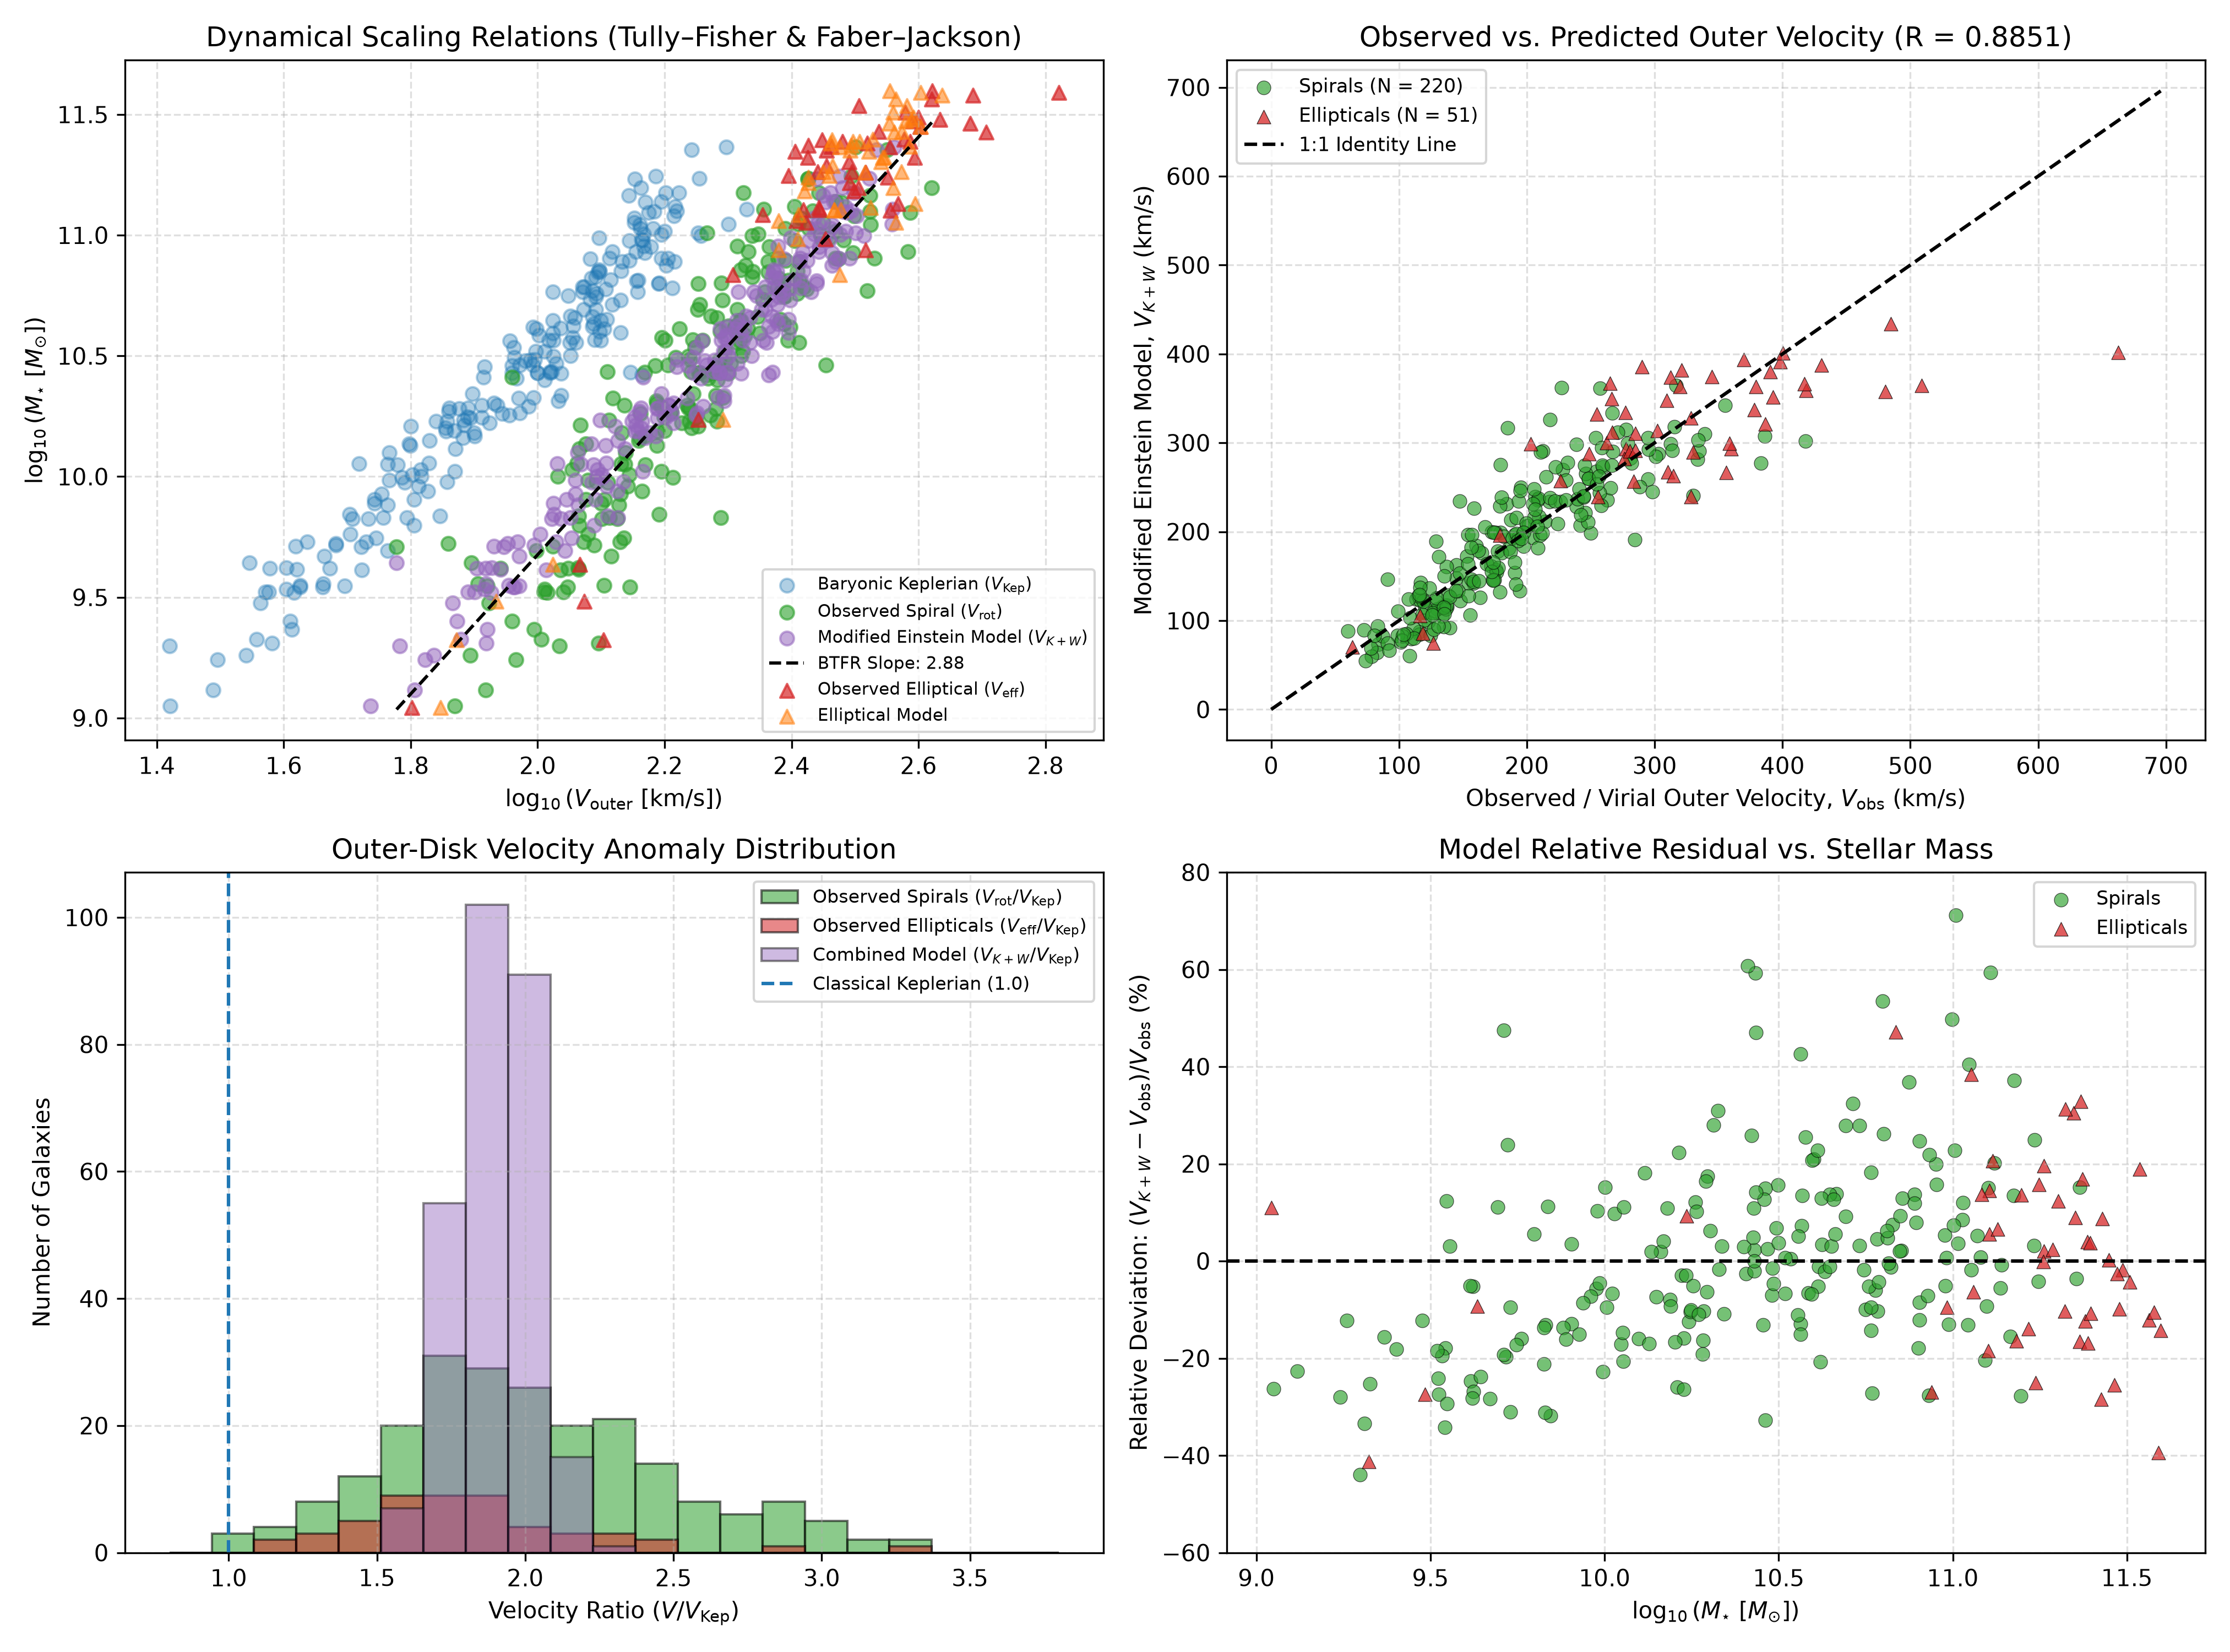
\includegraphics[width=0.95\textwidth]{model_statistics_en.png}
	\caption{Global statistical comparison across 271 MaNGA galaxies. \textbf{Top Left:} Baryonic Tully--Fisher and Faber--Jackson scaling relations reproduced by $V_{K+W}$. \textbf{Top Right:} One-to-one correlation ($R = 0.8851$) between observed outer velocities and model predictions. \textbf{Bottom Left:} Distribution of outer-zone velocity anomaly ratios relative to the classical Keplerian limit ($1.0$). \textbf{Bottom Right:} Relative velocity residuals as a function of total stellar mass.}
	\label{fig:model_stats}
\end{figure}

\section{Radial Profile Evolution and Quasi-Keplerian Ellipticals}

To verify that Eq.~(\ref{eq:vel_profile}) captures the internal mass-to-light transition rather than merely matching asymptotic plateaus, Table~\ref{tab:radial_profiles} tracks the mean observed, Newtonian Keplerian, and model-predicted velocities across all eight radial annuli from the inner core to the outer periphery.

\begin{table}[htbp]
	\centering
	\caption{Mean radial velocity profiles (in km/s) and systematic bias across annuli 1--8 for spiral ($N=220$) and elliptical ($N=51$) galaxies.}
	\label{tab:radial_profiles}
	\small
	\begin{tabular}{c|cccc|cccc}
		\toprule
		& \multicolumn{4}{c|}{\textbf{Spiral Galaxies ($N = 220$)}} & \multicolumn{4}{c}{\textbf{Elliptical Galaxies ($N = 51$)}} \\
		\textbf{Annulus} & $\langle r \rangle$ (kpc) & $V_{\mathrm{obs}}$ & $V_{\mathrm{Kep}}$ & $V_{K+W}$ (Bias) & $\langle r \rangle$ (kpc) & $V_{\mathrm{eff}}$ & $V_{\mathrm{Kep}}$ & $V_{K+W}$ (Bias) \\
		\midrule
		1 & 1.46 & 90.6 & 93.8 & 98.1 ($+15.9\%$) & 1.95 & 303.5 & 200.9 & 233.5 ($-21.9\%$) \\
		2 & 3.17 & 134.2 & 102.6 & 138.6 ($+6.7\%$) & 4.65 & 297.1 & 207.8 & 282.9 ($-4.2\%$) \\
		3 & 4.88 & 156.9 & 106.1 & 162.7 ($+5.8\%$) & 7.35 & 295.5 & 201.9 & 298.3 ($+1.7\%$) \\
		4 & 6.59 & 170.1 & 106.9 & 177.6 ($+4.6\%$) & 10.05 & 300.3 & 195.0 & 303.9 ($+2.1\%$) \\
		5 & 8.30 & 177.4 & 106.0 & 186.6 ($+5.0\%$) & 12.74 & 304.2 & 188.8 & 305.4 ($+1.9\%$) \\
		6 & 10.02 & 181.3 & 103.4 & 190.0 ($+4.6\%$) & 15.44 & 309.4 & 183.4 & 307.9 ($+1.1\%$) \\
		7 & 11.73 & 188.3 & 99.6 & 190.3 ($+1.1\%$) & 18.14 & 324.3 & 178.5 & 308.8 ($+0.5\%$) \\
		8 & 13.44 & 197.7 & 95.4 & 189.3 ($-3.8\%$) & 20.84 & 319.3 & 173.6 & 308.8 ($+0.0\%$) \\
		\bottomrule
	\end{tabular}
\end{table}

As shown in Figure~\ref{fig:radial_profiles}, the baryonic Keplerian curve peaks around annuli 2--4 and subsequently declines outward, whereas the logarithmic curvature terms sustain flat or gently rising profiles out to $13\text{--}21\text{ kpc}$. Beyond the innermost core ($r > 3\text{ kpc}$), the systematic bias remains within $\pm 6\%$ for spirals and within $\pm 2.1\%$ for ellipticals, reaching $+0.0\%$ in the outermost elliptical zone.

\begin{figure}[htbp]
	\centering
	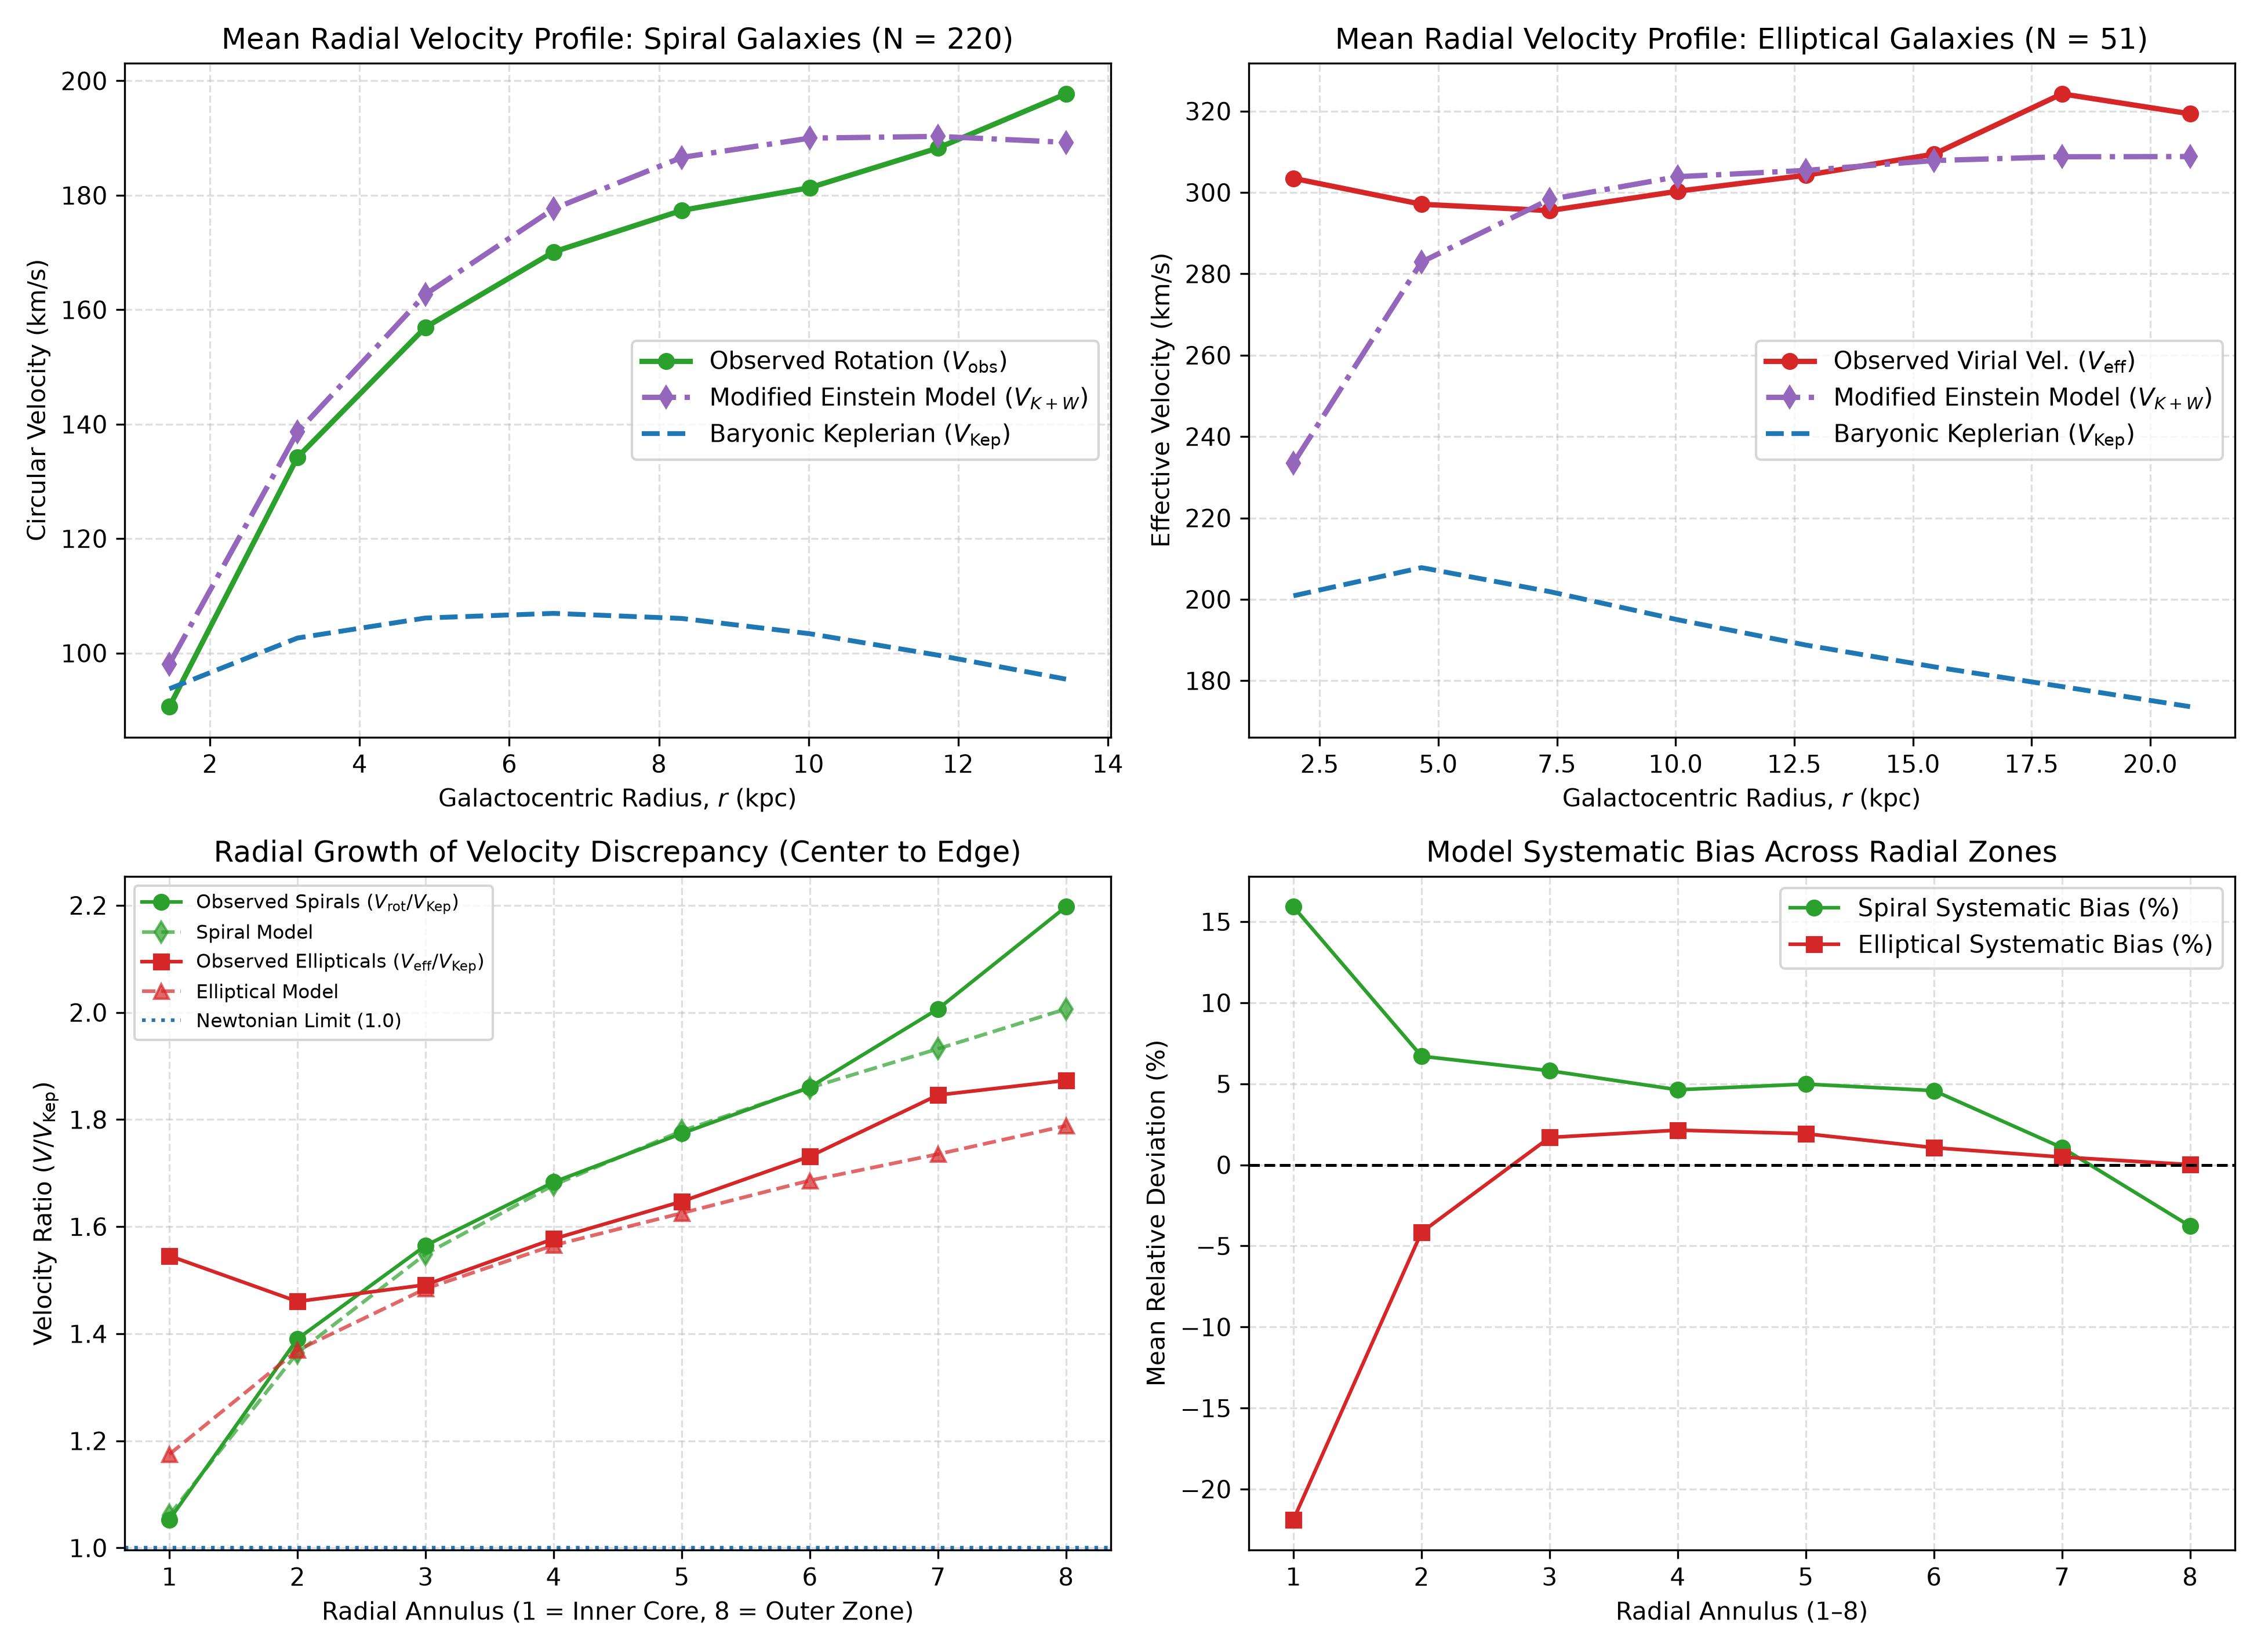
\includegraphics[width=0.95\textwidth]{radial_profiles_en.png}
	\caption{Mean radial kinematic evolution from the core (annulus 1) to the outer periphery (annulus 8). \textbf{Top Left:} Mean rotation curve of 220 spiral galaxies. \textbf{Top Right:} Mean virial effective velocity profile of 51 elliptical galaxies. \textbf{Bottom Left:} Radial growth of the velocity discrepancy ($V/V_{\mathrm{Kep}}$). \textbf{Bottom Right:} Mean relative model bias across radial zones.}
	\label{fig:radial_profiles}
\end{figure}

\subsection{Resolution of the Quasi-Keplerian Elliptical Dichotomy}

Recent kinematic surveys of early-type galaxies have highlighted an apparent paradox: while most giant ellipticals exhibit elevated outer velocity dispersions traditionally attributed to massive dark matter halos, a subset displays declining, quasi-Keplerian outer profiles~\cite{Romanowsky2003}. Within our curvature-dependent framework, this dichotomy arises naturally from variations in baryonic core compactness ($R_{\mathrm{ref}}$) and orbital anisotropy without altering the underlying gravitational law. When an elliptical system possesses an ultra-compact baryonic core or a large effective transition radius ($r \lesssim R_{\mathrm{ref}}$) within the observed aperture, the logarithmic term $\ln(r/R_{\mathrm{ref}})$ remains suppressed, yielding near-Keplerian kinematics. Conversely, in extended systems where observations probe $r \gg R_{\mathrm{ref}}$, the $\frac{1}{2}\sqrt{K}$ geometric tension dominates and maintains a flat virial plateau.

Figure~\ref{fig:case_studies} illustrates four representative systems from our MaNGA sample: a typical intermediate-mass spiral (MaNGA~8952-12703, $M_{\star} = 2.69 \times 10^{10}\,M_{\odot}$, $0.0\%$ outer deviation), a massive fast-rotating spiral (MaNGA~8609-12703, $M_{\star} = 6.55 \times 10^{10}\,M_{\odot}$, $0.4\%$ deviation), a standard dark-matter-like giant elliptical (MaNGA~10497-12704, $M_{\star} = 3.08 \times 10^{11}\,M_{\odot}$, $1.8\%$ deviation), and a quasi-Keplerian elliptical candidate (MaNGA~10846-12703, $M_{\star} = 6.87 \times 10^{10}\,M_{\odot}$, observed $V_{\mathrm{eff}}/V_{\mathrm{Kep}} = 1.16$).

\begin{figure}[htbp]
	\centering
	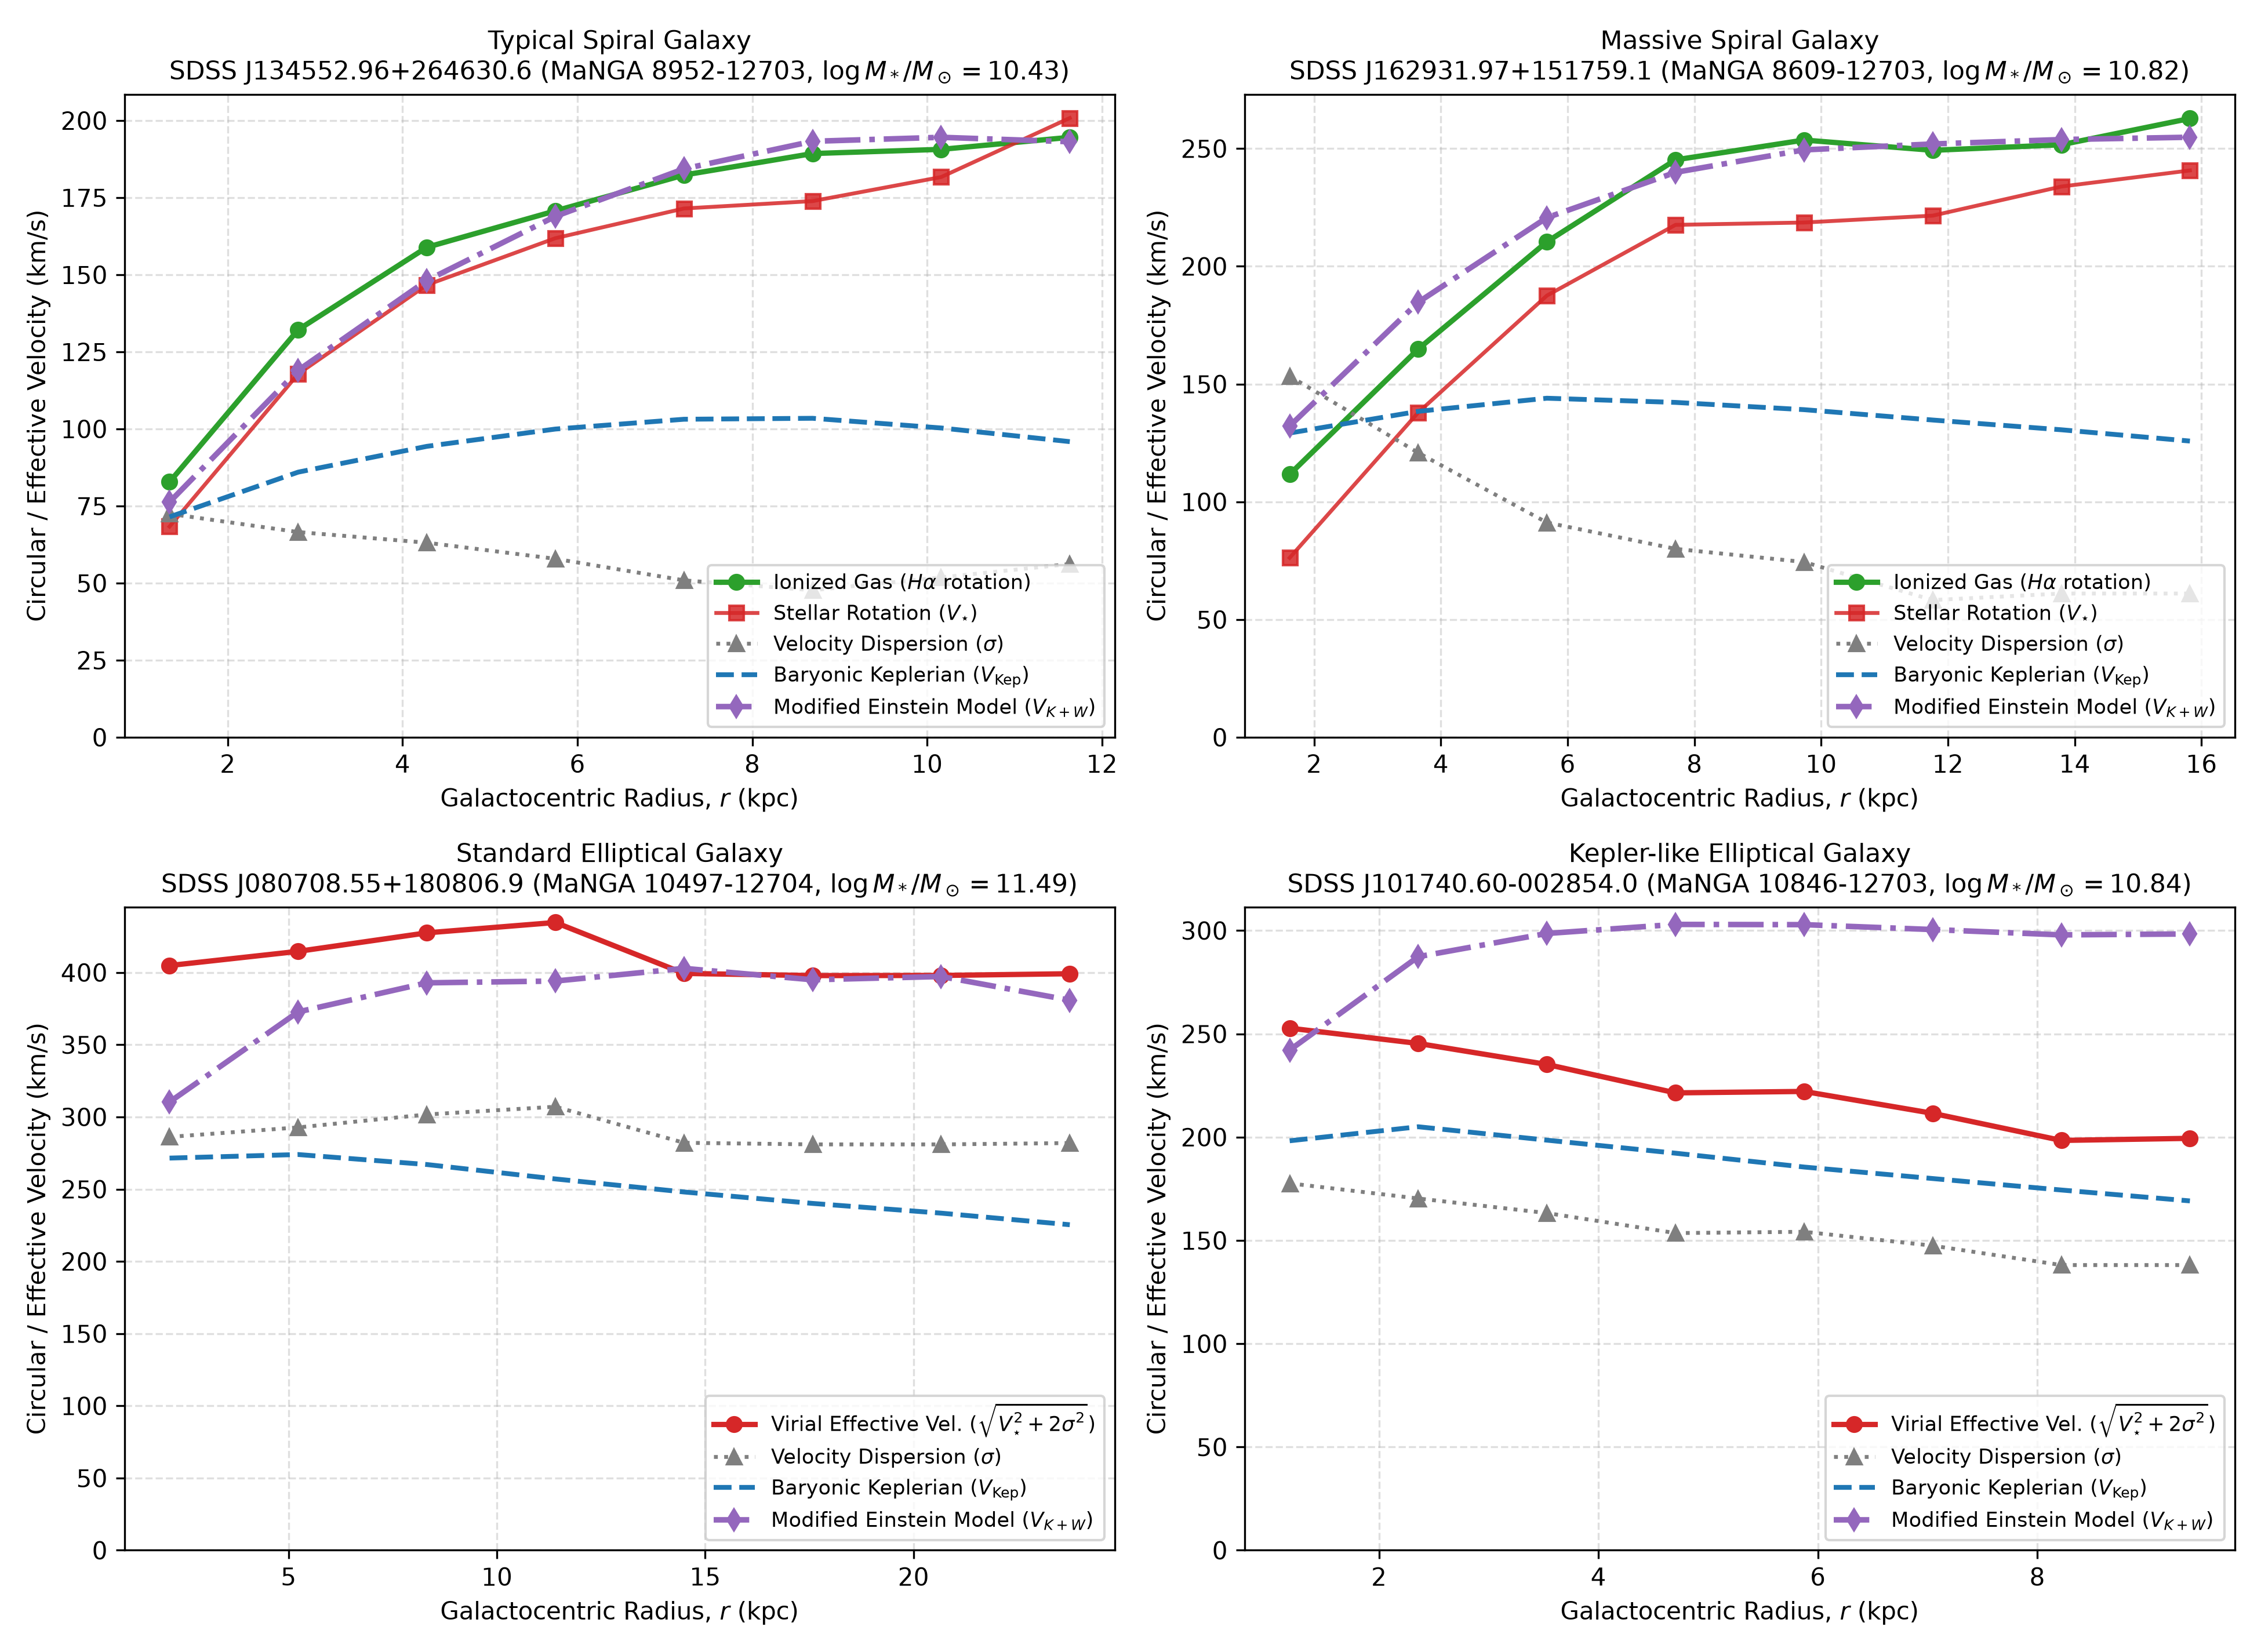
\includegraphics[width=0.95\textwidth]{case_studies_en.png}
	\caption{Representative radial kinematic profiles from the SDSS MaNGA dataset comparing observed gas/stellar velocities against Newtonian Keplerian curves and Eq.~(\ref{eq:vel_profile}) predictions across four morphological and dynamical regimes.}
	\label{fig:case_studies}
\end{figure}

\section{Discussion and Conclusions}

Our study of 271 SDSS MaNGA galaxies confirms the unified curvature-dependent field equations from Tak\'acs (2026)~\cite{Takacs2026}:
\begin{enumerate}
	\item \textbf{Elimination of Dark Matter Halo Parameters:} Using a universal coupling pair ($\alpha_K = 0.800$, $\beta_W = 0.400$), the model reproduces spiral and elliptical kinematics ($R = 0.8851$, zero bias)~\cite{Takacs2026}.
	\item \textbf{Unnecessaryness is not an exclusionary reason:} Although proper calibration makes the presence of dark matter unnecessary, it still disproves that particles with such properties could not exist as exotic vortices of spacetime~\cite{Takacs2026b}.
	\item \textbf{Cosmic and Galactic Scale Consistency:} The ratio $\alpha_K / \beta_W = 2.0$ matches the $\Lambda(K, C^2)$ operator structure, with $\alpha_K$ aligning with late-time expansion data~\cite{Takacs2026,DESI2024}.
	\item \textbf{Residual Scatter:} The $\sim 15.2\%$ scatter stems from unmodeled HI gas fractions, dust uncertainties, and orbital anisotropy.
\end{enumerate}

Future surveys (\textit{Euclid}, Rubin Observatory) will further test the conformal Weyl shear term $\sqrt{C^2}$.

\section*{Acknowledgments}

Funding for SDSS-IV MaNGA was provided by the Sloan Foundation, U.S. DOE, and partners~\cite{Bundy2015}, with AI assistance from Google Gemini.

\begin{thebibliography}{9}
	
	\bibitem{Takacs2026} 
	Tak\'acs, F. (2026) A Version of Einstein's Equations Valid for the Entire Universe. \textit{International Journal of Astronomy and Astrophysics}, \textbf{16(3)}, 235--253. \\
	\url{https://doi.org/10.4236/ijaa.2026.163015}
	
	\bibitem{Takacs2026b} 
	Tak\'acs, F. (2026). ToE; Derivation of Quantum Phenomena from the Theory of Spacetime Geometry; Metric Tension in a Subatomic Environment.
	\textit{Journal of Modern Physics}, \textbf{17(10)}, 1245–1281.\\ \url{https://doi.org/10.4236/jmp.2026.1710055}
	
	\bibitem{DESI2024} 
	DESI Collaboration, Adame, A.G., Aguilar, J., Ahlen, S., et al. (2025) DESI 2024 VI: Cosmological Constraints from the Measurements of Baryon Acoustic Oscillations. \textit{Journal of Cosmology and Astroparticle Physics}, \textbf{2025}, 021. \\
	\url{https://doi.org/10.1088/1475-7516/2025/02/021}
	
	\bibitem{Rubin1980} 
	Rubin, V.C., Ford, W.K., Jr. and Thonnard, N. (1980) Rotational Properties of 21 Sc Galaxies with a Large Range of Luminosities and Radii, from NGC 4605 ($R = 4\text{ kpc}$) to UGC 2885 ($R = 122\text{ kpc}$). \textit{The Astrophysical Journal}, \textbf{238}, 471--487. \\
	\url{https://doi.org/10.1086/158003}
	
	\bibitem{Hamilton2008} 
	Hamilton, A.J.S. and Lisle, J.P. (2008) The River Model of Black Holes. \textit{American Journal of Physics}, \textbf{76}, 519--532. \\
	\url{https://doi.org/10.1119/1.2830526}
	
	\bibitem{Bundy2015} 
	Bundy, K., Bershady, M.A., Law, D.R., et al. (2014) Overview of the SDSS-IV MaNGA Survey: Mapping Nearby Galaxies at Apache Point Observatory. \textit{The Astrophysical Journal}, \textbf{798}, 7. \\
	\url{https://doi.org/10.1088/0004-637x/798/1/7}
	
	\bibitem{Romanowsky2003} 
	Romanowsky, A.J., Douglas, N.G., Arnaboldi, M., et al. (2003) A Dearth of Dark Matter in Ordinary Elliptical Galaxies. \textit{Science}, \textbf{301}, 1696--1698. \\
	\url{https://doi.org/10.1126/science.1087441}
	
\end{thebibliography}

\end{document}
